% =====================================================================================================
\section{Discussion and Limitations}\label{sec:discussion}
\begin{figure}[t]
\centering
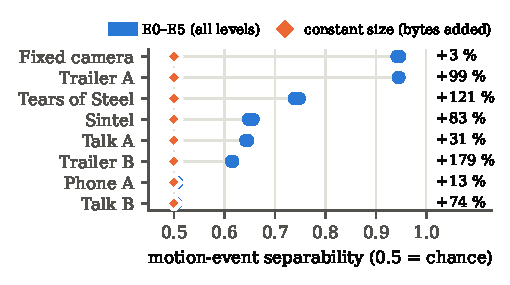
\includegraphics[width=\columnwidth]{figures/fig_size_channel.pdf}
\caption{Motion events detected from frame sizes alone, for every protection level (bar: E0--E5 range) and with every frame padded to a constant size (diamond; bytes added on the right). Fixed camera: synthetic scene; the others are the real clips.}
\label{fig:size}
\end{figure}
% generated by paper/make_assets.py from paper/data -- do not edit
\begin{table}[t]
\caption{Which of 7 videos is playing, identified from $W$ consecutive encrypted frame sizes (after~\cite{schuster2017}), in \% of 300 queries; chance 14\,\%. At 10 frames/s, $W{=}10$ is one second. Bytes: cost over the E2 stream.}
\label{tab:fingerprint}
\centering\small
\resizebox{\columnwidth}{!}{%
\begin{tabular}{lrrrrr}
\toprule
Stream & Bytes & $W{=}5$ & $W{=}10$ & $W{=}30$ & $W{=}100$ \\
\midrule
E1--E4 & +0\,\% & 76 & 98 & 100 & 100 \\
E5 & +12\,\% & 69 & 99 & 100 & 100 \\
pad to 1\,KB & +6\,\% & 21 & 40 & 85 & 97 \\
pad to running max. & +55\,\% & 18 & 23 & 31 & 46 \\
pad to 10\,s max. & +41\,\% & 18 & 31 & 52 & 95 \\
constant size & +81\,\% & 14 & 13 & 19 & 14 \\
\bottomrule
\end{tabular}}
\end{table}

\textit{What no level hides.} Encryption hides content, not length. Frame sizes reveal motion at every level alike (Fig.~\ref{fig:size}). They also identify a known video, as Schuster et al.\ showed for encrypted streaming~\cite{schuster2017}: an attacker who encodes candidate videos himself and correlates the size sequence picks the right one of \FpVideos{} videos from ten frame sizes \FpEtwoTen\,\% of the time under E1--E4 and \FpEfiveTen\,\% under E5 (chance \FpChance\,\%, Table~\ref{tab:fingerprint}). Padding to 1\,KB steps lowers that to \FpKbTen\,\% for $+$\FpKbCost\,\% bytes but not over 100 frames (\FpKbHundred\,\%), padding to the running maximum to \FpRunTen\,\% for $+$\FpRunCost\,\%, and only constant-size frames reach chance, at $+$\FpConstCost\,\% on these edited clips. Constant-size frames close the channel cheaply for a fixed camera ($+$\PadFixed\,\%) but cost up to $+$\PadFilmMax\,\% bytes on edited clips; padding to the largest frame so far gives a separability of \PadRunSep{} for $+$\PadRunCost\,\% on the fixed camera (\PadRunFilmSepMin--\PadRunFilmSepMax{} on the real clips), while bitrate regulation lets up to \RcPadOverMax\,\% of frames exceed a cap. A surveillance camera is the favourable case: its scene is fixed and padding is cheap.

\textit{Limitations.} Five limitations bound our claims. First, the board confirms correctness but not yet speed or power: the encoder is bit-exact on the PYNQ-Z2, but our frame rate there is set by a Python driver on the ARM, the fabric-only time and the power are not yet measured on the board, and the power figures come from simulated switching activity; whether DDR feeds the four-lane encoder its \RtlFourLanesInMBs\,MB/s of pixels is also open. Second, sign and amplitude encryption leak outlines by construction (Lemma~\ref{lem:format}), however many bits are encrypted; only a change of block positions removes them, at a bitrate cost. Third, frame sizes leak at every level, as above. Fourth, our attackers are greedy or trained on a few clips; stronger puzzle solvers or attackers trained on large video corpora may extract more from E5, and a trained network already undoes sign-only encryption (E1). Fifth, the master key is pre-shared; a key exchange such as X25519 on the ARM core at session start, as DTLS-SRTP does for SRTP~\cite{rfc3711}, would remove that assumption without touching the fabric. On the protocol side, the receiver cannot tell heavy benign loss from partial jamming, so only near-total suppression escalates, and the reaction time is bounded below by the one-second decision window.

\textit{Reproducibility and data.} Every number in this paper is produced by a script from stored results and inserted into the text by a generator, never typed; a test fails if a table in the manuscript differs from what the data produce. The open sources (the Blender Foundation films and the Kodak images) can be downloaded and rerun; the private clips are identified by SHA-256 hash and never shown, and frames of them are never stored as images. The golden model, the RTL, the testbenches, the Vivado and board scripts, the experiment scripts and the scripts that rerun all GPU and long-CPU experiments in one cloud session are available in our repository.

\textit{Lessons.} Three kinds of error recurred while building this system, and each changed how we work. Simulation-only success hid timing problems that only place and route exposed, so post-route numbers are now part of every hardware claim. Experiment scripts were wrong more often than the RTL: a set point that clips opening on black could not reach, an estimator that wound up when its input saturated, a controller tuned at one operating point and unstable at another, and a test source that stamped the wall-clock time into every frame. Each was found because a result looked implausible on new data, and each now has a regression test. Finally, two claims had to be withdrawn when stronger evidence arrived: the E5 edge correlation of the U-Net is above that of the plain prior once more data is used, which the frame-statistics control explains, and the cost of hiding frame sizes is small only for fixed cameras.

\textit{Ethics.} The clips with identifiable people are used only to measure what an eavesdropper could recover; no picture derived from them appears here, and none is stored.

% =====================================================================================================
\section{Conclusion}\label{sec:conclusion}
Encrypting coefficient signs and amplitudes with Ascon inside a JPEG encoder costs no cycles, provably keeps every protection level playable, and, combined with a per-frame tag over metadata and scan, turns a plain MJPEG stream into an authenticated one. Field encryption alone, however, leaves the outline of the scene to anyone who counts non-zero coefficients, and published format-compliant schemes also fall to one known frame because their key material does not change. A keyed permutation of macroblocks that is drawn anew for every frame removes the outline under every attack we could build, and with restart segments it fits in hardware without a frame buffer: the fabric codes and authenticates the segments, the processor only reorders them. Parallel lanes over the same segments raise throughput to \RtlFourLanesMpix\,Mpixel/s at 100\,MHz, and a closed feedback loop answers active network attacks within about a second in simulation. No level hides frame sizes, which identify a known video and reveal motion; constant-size frames close that channel at a cost that is small only for fixed cameras. Next are the fabric-only time and power on the board, a driver that keeps the ARM off the pixel path, size padding in hardware, a shared Ascon core across lanes, a 125\,MHz clock, key derivation with the standard's extendable-output function, and a key exchange at session start.
